% !TEX ROOT=./main.tex



\section{Numerical Experiments}



\subsection{Strongly Convex}

\begin{figure}[h!]
\centering
\begin{tabular}{cc}
	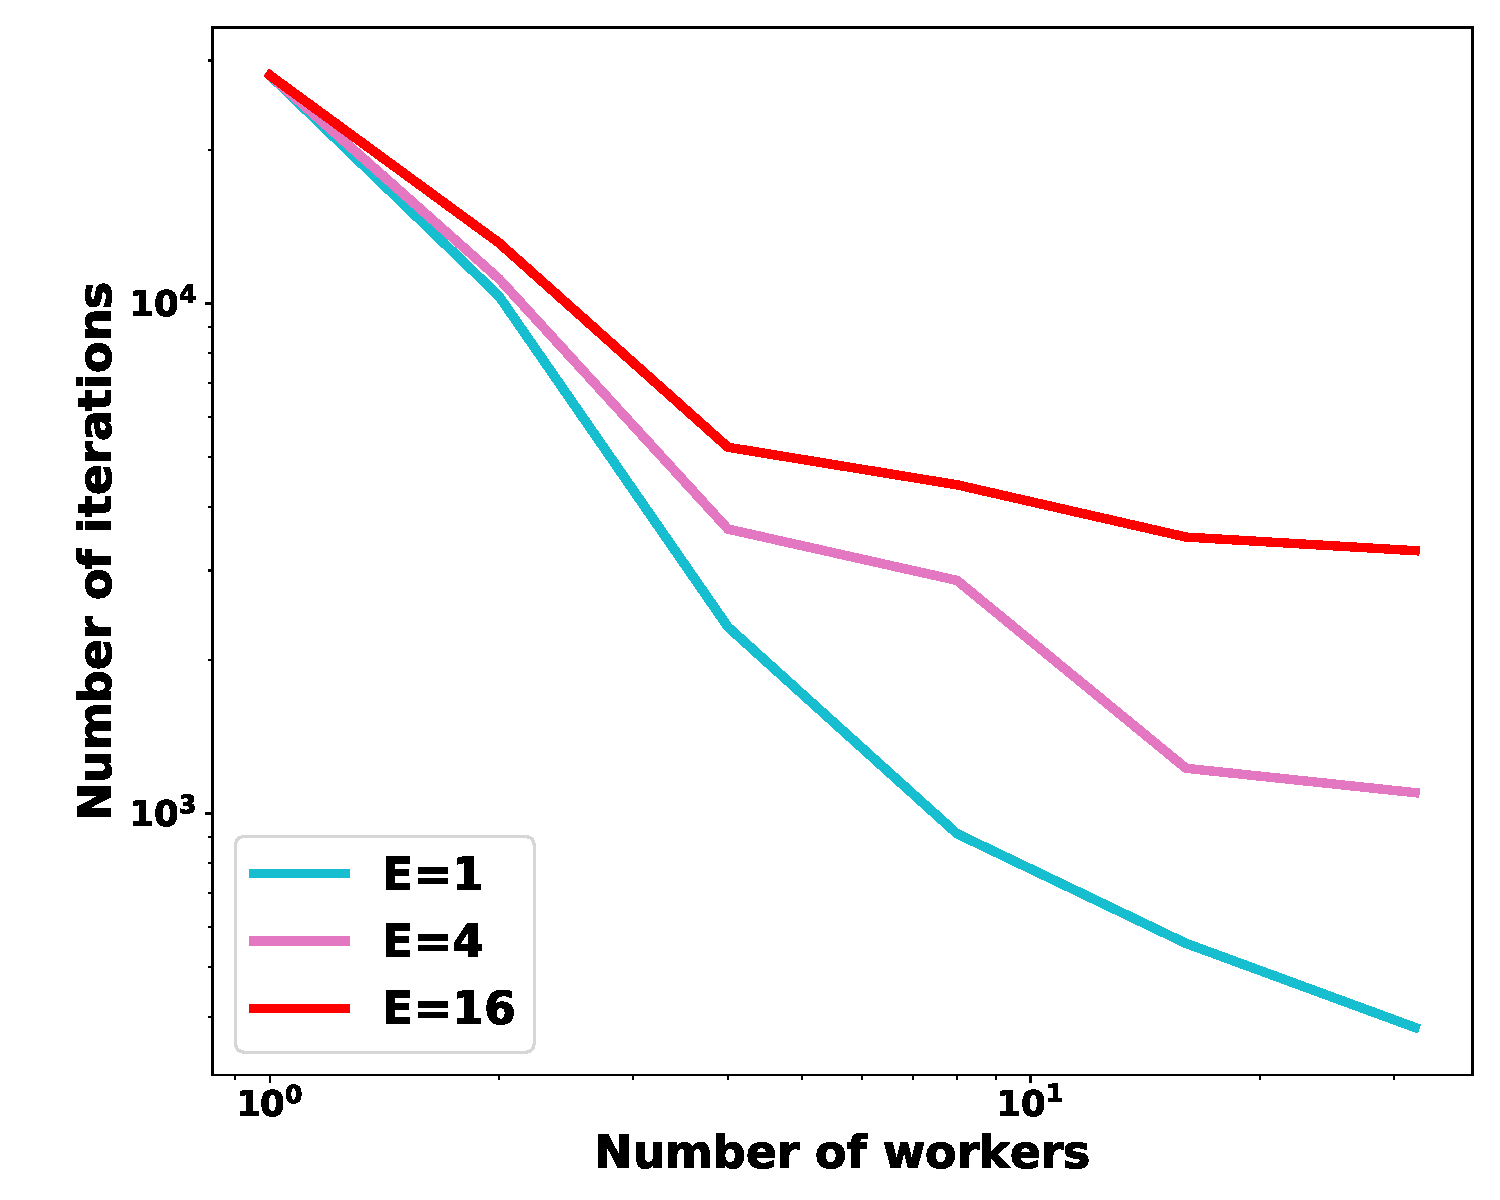
\includegraphics[width=0.45\textwidth]{fig/paper-stronglycvxsmthspeedupNodesT-min-w8a-epsilon0131-reg1e-05.pdf} & 
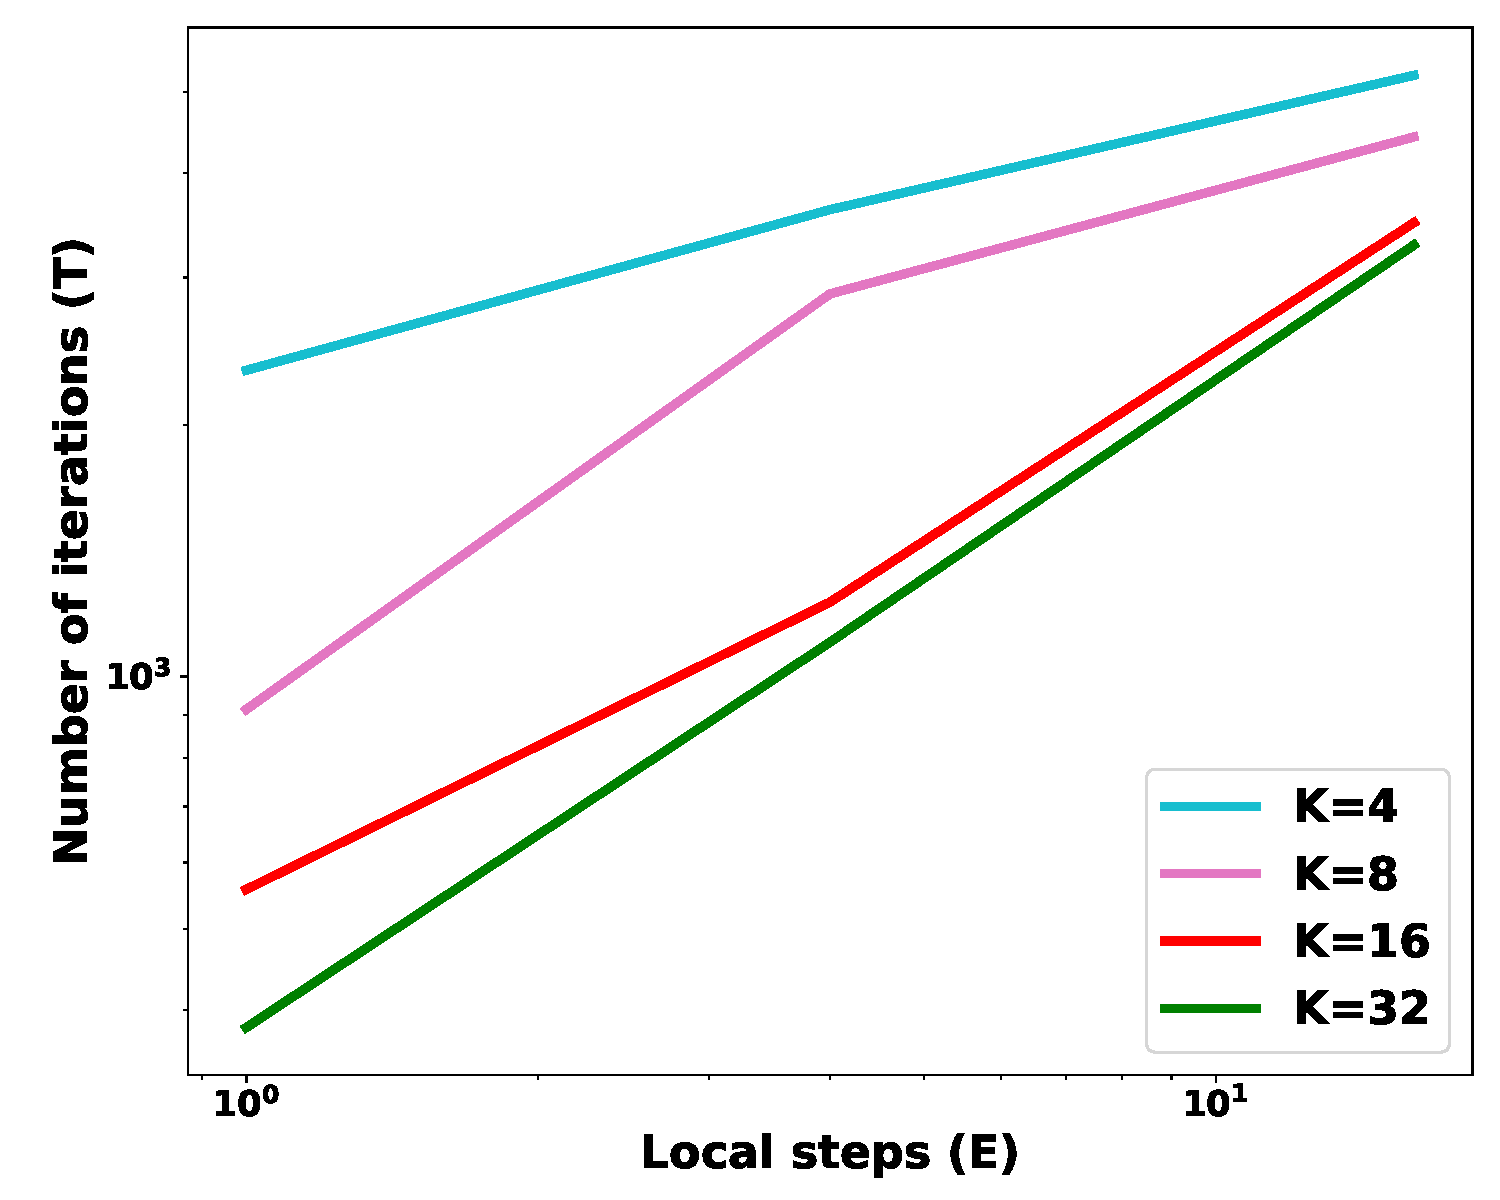
\includegraphics[width=0.45\textwidth]{fig/paper-stronglycvxsmthspeedupEpochsT-min-w8a-epsilon0131-reg1e-05.pdf} \\
\end{tabular}
	\caption{Logistic regression with regularization $1e-5$. The linear speed up w.r.t the number of nodes and number of epochs. The synthetic dataset has $N=49749$ samples, evenly distributed on $1, 2, 4, 8, 16, 32$ devices. The figure shows the number of iterations/rounds needed to converge to $\epsilon-$accuracy, where $\epsilon=0.005$. The learning rate is decayed as the $\eta_t = \min(32, \frac{Nc}{1 + t})$, where we extensively search the best learning rate $c \in \{2^{-1}c, 2^{-2}c, c, 2c, 2^{2}c\}$ and for each configuration. Batch size is 4 in this case.}
\end{figure}



\subsection{Convex smooth objective}

\begin{figure}[h!]
\centering
\begin{tabular}{cc}
	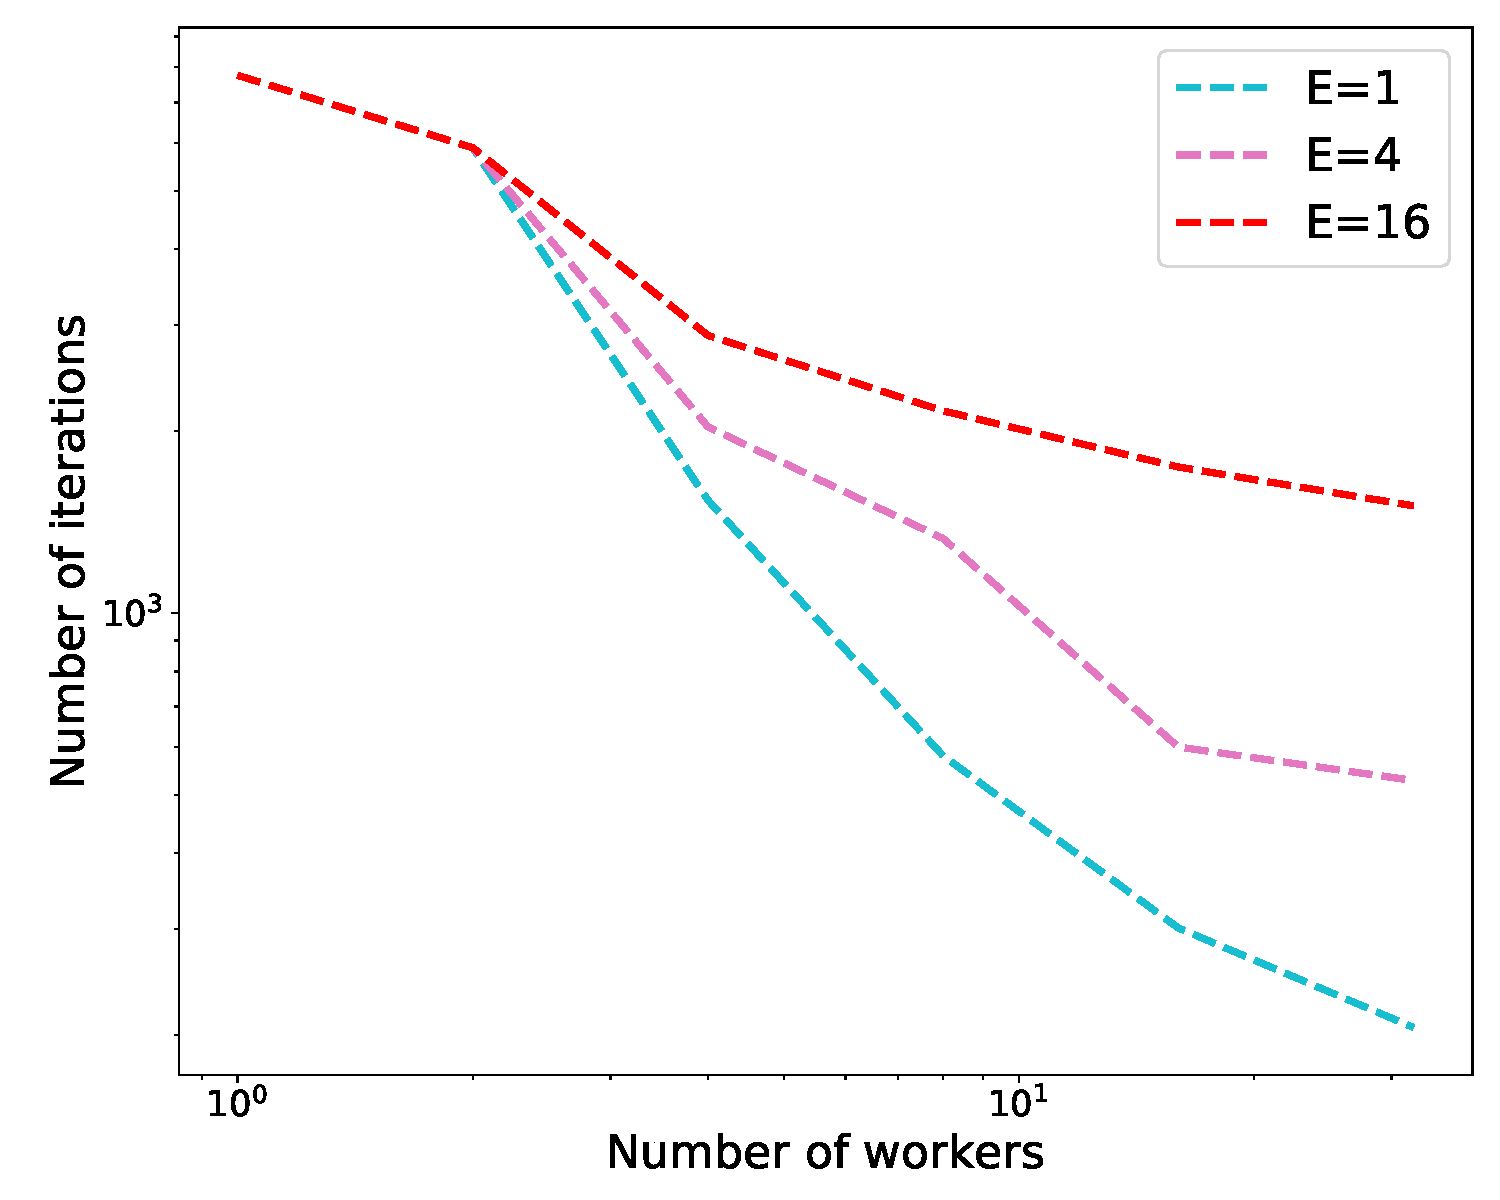
\includegraphics[width=0.45\textwidth]{fig/paper-cvxsmoothspeedupNodesT-min-w8a-epsilon013-b4-reg0.pdf} & 
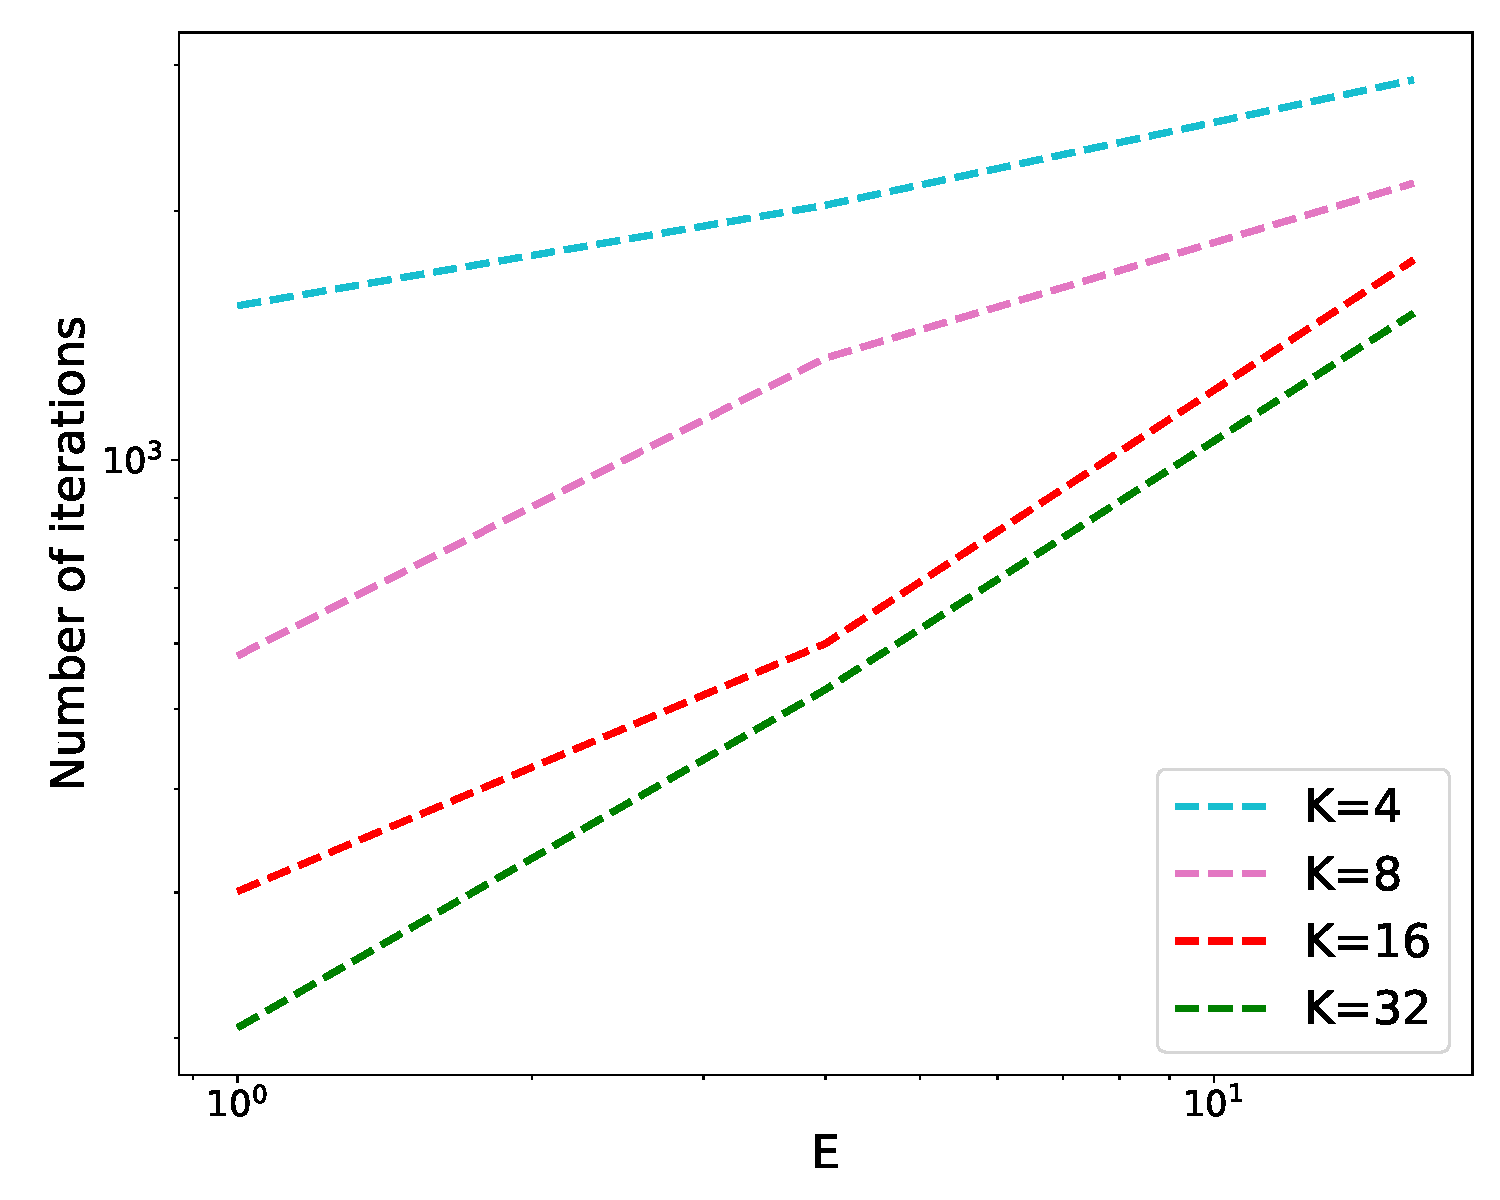
\includegraphics[width=0.45\textwidth]{fig/paper-cvxsmoothspeedupEpochsT-min-w8a-epsilon013-b4-reg0.pdf} \\
\end{tabular}
	\caption{Logistic regression without regularization. The linear speed up w.r.t the number of nodes and number of epochs. The w8a dataset has $N=49749$ samples, evenly distributed on $1, 2, 4, 8, 16, 32, 64, 128, 256, 512, 1024$ devices. The figure shows the number of iterations needed to converge to $\epsilon-$accuracy, where $\epsilon=0.02$. The learning rate is decayed as the $\eta_t = \min(\eta_0, \frac{Nc}{1 + t})$, where we extensively search the best learning rate $c \in \{2^{-1}c, 2^{-2}c, c, 2c, 2^{2}c\}$, $\eta_0 \in \{1, 32\}$ and for each configuration. Batch size is 4 in this case.}
\end{figure}




\subsection{Linear regression}





